\documentclass[czech,12pt,a4paper,titlepage]{article}
\usepackage[left=20mm,right=20mm,top=25mm,bottom=25mm]{geometry}
\usepackage[autostyle]{csquotes}
\usepackage[export]{adjustbox}
\usepackage[czech]{babel}
\usepackage{graphicx}

\title{%
    \textbf {Match to win} \\
    \large Seznamovací aplikace pro hráče}
\author{Kateřina Baierová}
\date{}

\begin{document}

\graphicspath{ {./img/} }

\begin{titlepage}
    \maketitle
    \thispagestyle{empty}
\end{titlepage}

\tableofcontents

\clearpage

\subsection*{Historie verzí dokumentu}

\bigskip
\bigskip
\bigskip

\begin{center}
    \begin{tabular}{ |c|c|c| }
        \hline
        Datum     & Změny                               & Verze \\
        \hline
        15.3.2023 & Specifikace zadání, FURPS, Use Case & 0     \\
        \hline
        23.3.2023 & Use Case scénáře                    & 1     \\
        \hline
        29.3.2023 & Úprava Use Case diagramu (extend)   & 1.1   \\
        \hline
        7.4.2023  & Class diagram                       & 2     \\
        \hline
        17.4.2023 & Úprava class diagramu               & 2.1   \\
        \hline
        21.4.2023 & Sekvenční diagramy                  & 3     \\
        \hline
        28.4.2023 & Aktivitní a stavové diagramy        & 4     \\
        \hline
    \end{tabular}
\end{center}

\clearpage

\section{Počáteční popis}

\subsection{Zadání od zákazníka}
Vytvořit mobilní aplikaci pro herní komunitu, která bude sloužit k nalezení odpovídajícího spoluhráče
pomocí zadání svých herních informací a požadavků (např. název hry, role, rank, preference hovoru nebo
pouze zpráv apod.), což by mělo vést dle zákazníka k lepšímu výkonu ve hře. Aplikace by měla být prospěšná
také pro e-sportové týmy, které se tam taktéž můžou zaregistrovat a hledat případné spoluhráče do svého týmu.

Jakmile dojde ke shodě mezi uživateli, automaticky se druhý profil přidá do seznamu přátel. Když si tento
seznam uživatel zobrazí, uvidí jednoduchý přehled uživatelských jmen a ikonku hry, ve které se shodli.
Tento seznam jde filtrovat podle jména, druhu hry nebo času přidání.

Následně by aplikace měla obsahovat také chat mezi hráči, popřípadě skupinový chat mezi účastníky týmu.
Nebude však obsahovat možnost nastavení pohlaví a profilového obrázku.
Alternativou bude výběr charakteru ze zaregistrovaných her.

\subsection{Důvod, okolnosti zavedení řešení}

Cílem tohoto softwarového projektu je vyvinout aplikaci, která bude sloužit jako příležitost pro hráče najít
si nejen skvělé spoluhráče, kteří budou na stejném nebo podobném herním levelu jako oni, ale také jako možnost
se seznámit s lidmi se stejnými zájmy.

Hlavní featurou této aplikace je rozmanitost ve výběru her a vlastní nastavení požadavků na spoluhráče.
Aplikace vám tedy bude ukazovat pouze hráče dle vašeho výběru, kterým vy osobně také vyhovujete.
\clearpage

\section{Systémové požadavky}

\subsection{Funkčnost (functionality - F)}

Tato sekce se zaměřuje na popis schopností (chování) systému.

\begin{enumerate}
    \item Aplikace musí umět správně vytvářet uživatelské profily dle výběru registrace uživatelem (Gamer/E-sport team).
    \item Aplikace musí umět rozeznat různé statistiky z několika her z profilů.
    \item Aplikace musí správně a co nejrychleji najít shodné profily vzhledem k zadaným požadavkům obou stran.
    \item Aplikace musí poskytnout informaci uživateli o jakékoliv nové shodě, zprávě nebo jiné změně na profilu.
    \item Aplikace musí uživatele správně upozornit na nedostatky/chyby na profilu, které mohou vést k
          neúspěšným nebo žádným shodám (při nevyplnění).
\end{enumerate}

\subsection{Vhodnost k použití (usability - U)}

Tato sekce specifikuje požadavky spojené s UX (user experience).

\begin{enumerate}
    \item Aplikace je určena pouze na mobilní telefony nebo tablety.
    \item Systém by měl pracovat ve více jazycích. Při uvedení do chodu, krom češtiny, také v angličtině. Mělo by
          se počítat s možností budoucího přidání více jazyků.
    \item Uživatel bude mít možnost světlého i tmavého režimu aplikace.
\end{enumerate}

\subsection{Spolehlivost (reliability- R)}

Tato sekce definuje nutnou míru spolehlivosti a zmiňuje případné záložní systémy.

\begin{enumerate}
    \item Systém nesmí být nedostupný více než 24 hodin.
    \item Všechna data systému musí být pravidelně zálohována.
\end{enumerate}

\subsection{Výkon (performance - P)}

Tato sekce popisuje metriky jako rychlost odezvy a maximální možný počet uživatelů.

\begin{enumerate}
    \item Systém musí zvládnout nápor několika tisíc současně přihlášených uživatelů. (budoucí nárůst)
    \item Systém musí být schopný reagovat do pěti sekund.
    \item Aplikaci budou schopna využívat veškerá mobilní zařízení. (IOS i Android)
\end{enumerate}

\subsection{Schopnost být udržována (supportability - S)}

Tato sekce se zabývá údržbou systému, která zahrnuje například záplaty, aktualizace s případnou
novou funkcionalitou a možnosti testování těchto novinek.

\begin{enumerate}
    \item Systém bude podporovat automatické aktualizace za předpokladu připojení na wifi (lze změnit v nastavení).
    \item Systém musí mít možnost testovat případnou novou funkcionalitu nebo záplaty na opravu chyb v neprodukčním prostředí.
    \item Klientská aplikace bude přizpůsobena všem mobilním zařízením.
\end{enumerate}

\section{Charakteristika aktérů a prostředí}

\subsection{Uživatelé figurující v systému}

\subsubsection*{Developer team}

Stará se o chod aplikace, její aktualizování a přidávání nových prostředků. V systému má
všechna oprávnění. Také řeší nahlášené profily a podle závažnosti rozesílá upozornění
nebo dané profily spolu s údaji maže a přesouvá na černou listinu.

\subsubsection*{Gamer}

Uživatel \textbf{Gamer} se vytvoří v aplikaci pomocí registrace pro hráče. Jeho oprávnění jsou
omezená. Může upravovat vlastní profil nebo kontaktovat profil jiný, se kterým má tzv. shodu (match).

\subsubsection*{E-sport team}

Uživatel \textbf{E-sport team} se vytvoří v aplikaci pomocí registrace pro týmy. Jeho oprávnění jsou
taktéž omezená, ale na rozdíl od Gamerů může kontaktovat kohokoliv kdykoliv. Také má možnost
založit skupinový chat, kde může pozvat jakékoliv uživatele z řádu Gamer.

\clearpage

\section{Scénáře případů použití systému}

\subsection{Ideální případ použití}

Uživatel se přihlásí pomocí svého uživatelského jména a hesla.\\ \\
Uživatel vyplní detailně všechna pole v profilu dle daných instrukcí.
Následně mu systém bude nacházet profily, které se shodují s jeho požadavky a zároveň on jejich.

\subsection{Hraniční případ použití}

Uživatel zapomněl své uživatelské jméno nebo heslo. V případě problému s heslem mu systém
navrhne možnost zapomenuté heslo, kde si heslo pomocí emailu může změnit. Pokud se jedná o
zapomenuté uživatelské jméno, je možnost se přihlásit pomocí emailu a hesla. \\ \\
Pokud uživatel nezadá své preference na spoluhráče, systém automaticky bere, že mu na tomto
faktoru nezáleží a budou mu vygenerované veškeré profily, kterým vyhovují jeho statistiky.

\subsection{Případ použití za hranou}

Uživatel zapomněl jak heslo, tak také email, kterým se v aplikaci registroval. V tomto
případě bohužel není možné se do aplikace přihlásit. \\ \\
Jestliže uživatel nevyplní svoje herní statistiky nebo nevyplní hry, ve kterých hledá
spoluhráče, systém tohoto uživatele nezařadí mezi potenciální spoluhráče ke kontaktování.

\clearpage

\section{Podrobný náhled na stavbu produktu}

\subsection{Use case diagram}

Níže přiložený use-case diagram (česky diagram případu užití) slouží k bližší ilustraci toho,
jak bude systém implementován v praxi.

\bigskip
\bigskip
\bigskip
\bigskip
\bigskip
\bigskip


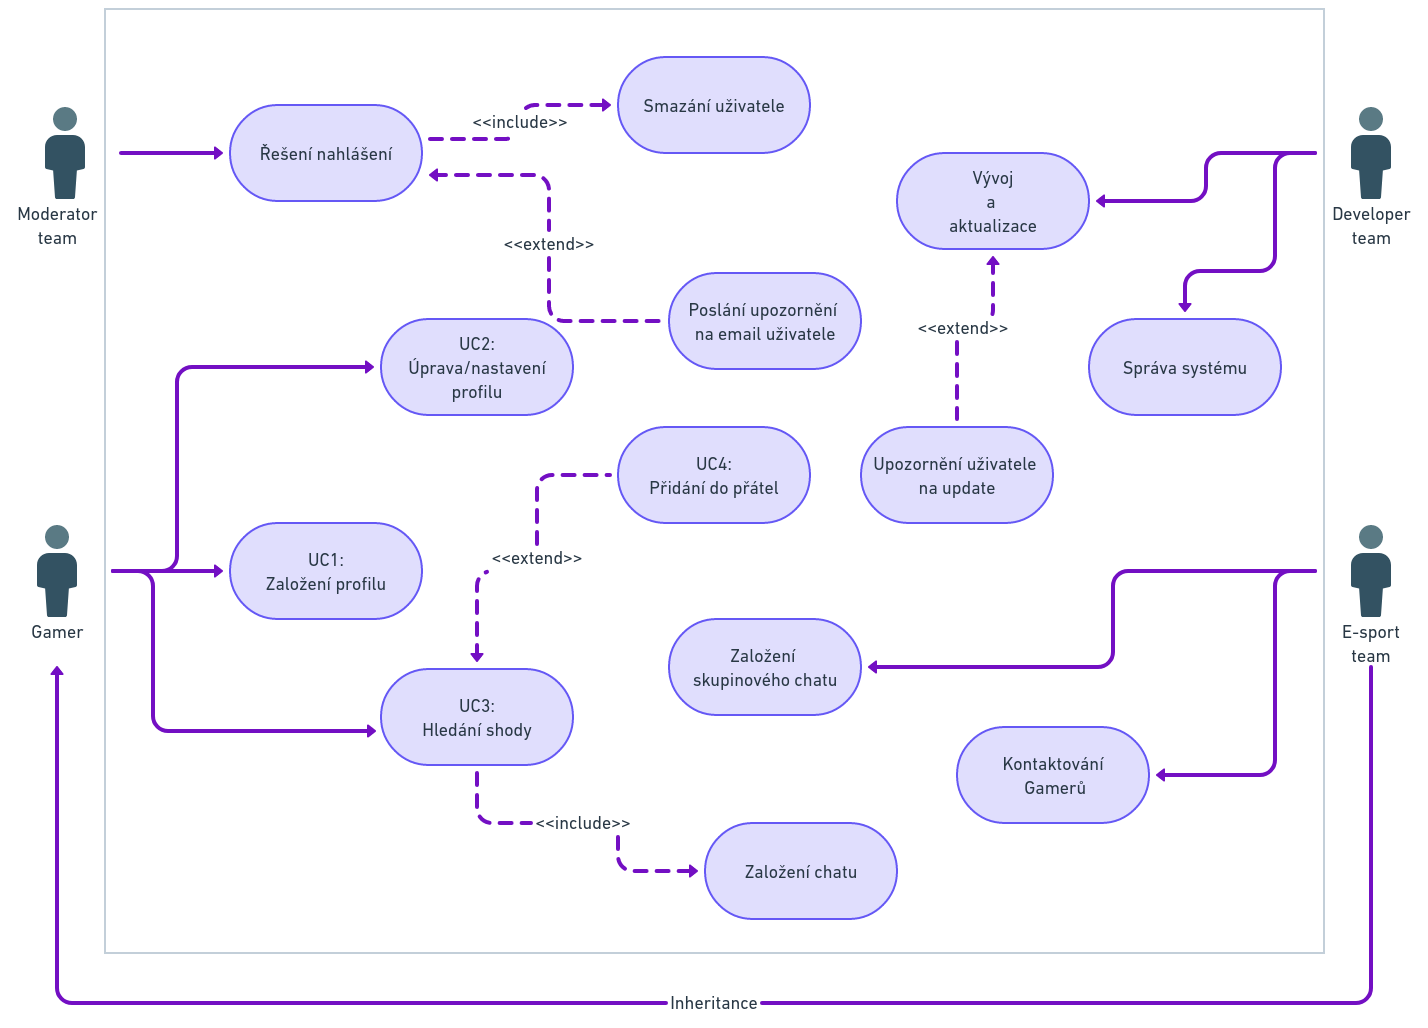
\includegraphics[width=1\textwidth, center]{UC_diagram.png}

\clearpage

\subsection{Konkrétní implementace use case 1}

\subsubsection{UC1: Parametry}

\begin{itemize}
    \item \textbf{Název:} Založení profilu uživatelem
    \item \textbf{Kontext:} Vytvoření nového profilu uživatelem
    \item \textbf{Primary actor:} Gamer nebo E-sport team
    \item \textbf{Precondition:} Uživatel nesmí mít již existující účet
    \item \textbf{Minimal guarantee:} Při chybě bude zobrazena chybová hláška
          \begin{itemize}
              \item Uživatelské jméno je již zabrané.
              \item Heslo nesplňuje minimální požadavky.
              \item Nedošlo k ověření emailové adresy.
          \end{itemize}
    \item \textbf{Success guarantee:} Nový profil je vytvořen
    \item \textbf{Trigger:} Uživatelská akce
\end{itemize}

\subsubsection{UC1: Hlavní scénář}

\begin{enumerate}
    \item Uživatel vybere jednu z možností registrace (pro hráče nebo týmy)
    \item Zadá nepoužívané uživatelské jméno
    \item Zadá svůj email k ověření
    \item Zadá 6místné heslo dle podmínek (alespoň 1 velké písmeno a číslo)
    \item Následně mu bude zobrazeno upozornění o potvrzení emailu
    \item Po úspěšném potvrzení emailu bude uživatel přesměnrovám na svůj nový profil
\end{enumerate}

\subsubsection{UC1: Extension}

\begin{enumerate}
    \item Pokus uživatel zadá již používané uživatelské jméno, zobrazí
          se mu chybové oznámení s návrhy podobných volných uživatelských jmen
    \item Pokud uživatel zadá falešný email (nedojde k ověření), jeho profil nebude vytvořen
\end{enumerate}

\clearpage

\subsection{Konkrétní implementace use case 2}

\subsubsection{UC2: Parametry}

\begin{itemize}
    \item \textbf{Název:} Úprava profilu uživatelem
    \item \textbf{Kontext:} Uživatel si chce změnit informace nebo požadavky na profilu
    \item \textbf{Primary actor:} Gamer nebo E-sport team
    \item \textbf{Precondition:} Uživatel musí být přihlášen
    \item \textbf{Minimal guarantee:} Při chybě bude zobrazena chybová hláška
          \begin{itemize}
              \item Chybí informace.
          \end{itemize}
    \item \textbf{Success guarantee:} Nová data jsou vložena
    \item \textbf{Trigger:} Uživatelská akce
\end{itemize}

\subsubsection{UC2: Hlavní scénář}

\begin{enumerate}
    \item Uživatel otevře svůj prpofil v aplikaci
    \item Vybere možnost "Úprava profilu"
    \item Vyplní nebo změní informace
    \item Uloží změny
\end{enumerate}

\subsubsection{UC2: Extension}

\begin{enumerate}
    \item Pokud uživatel nezadá všechny potřebné informace, údaje nebudou
          uloženy a bude upozorněn  na problém
\end{enumerate}

\clearpage

\subsection{Konkrétní implementace use case 3}

\subsubsection{UC3: Parametry}

\begin{itemize}
    \item \textbf{Název:} Hledání shody s jiným profilem
    \item \textbf{Kontext:} Uživatel hledá spoluhráče
    \item \textbf{Primary actor:} Gamer
    \item \textbf{Precondition:} Uživatel je přihlášen a má vyplněné informace o sobě a své preference
    \item \textbf{Minimal guarantee:} Při chybě bude zobrazena chybová hláška
          \begin{itemize}
              \item Bohužel žádná shoda
          \end{itemize}
    \item \textbf{Success guarantee:} Systém uživateli najde shodné profily k vybrání
    \item \textbf{Trigger:} Uživatelská akce
\end{itemize}

\subsubsection{UC3: Hlavní scénář}

\begin{enumerate}
    \item Uživatel vybere ikonu hledání shody v aplikaci
    \item Systém mu začne nacházet shodné profily
    \item Uživatel si vybírá, jestli si chce navržený profil přidat do
          přátel (přesunutím doprava) nebo ne (doleva)
\end{enumerate}

\subsubsection{UC3: Extension}

\begin{enumerate}
    \item Pokud uživatel přesune doprava prodil, který už předtím
          přesunul uživatelův profil doprava, objeví se upozornění na shodu
          a automaticky se vytvoří společný chat
\end{enumerate}

\clearpage

\subsection{Class diagram}

Tento diagram popisu je strukturu celého systému. Každá třída má své atributy a funkce.

\bigskip
\bigskip
\bigskip
\bigskip
\bigskip
\bigskip


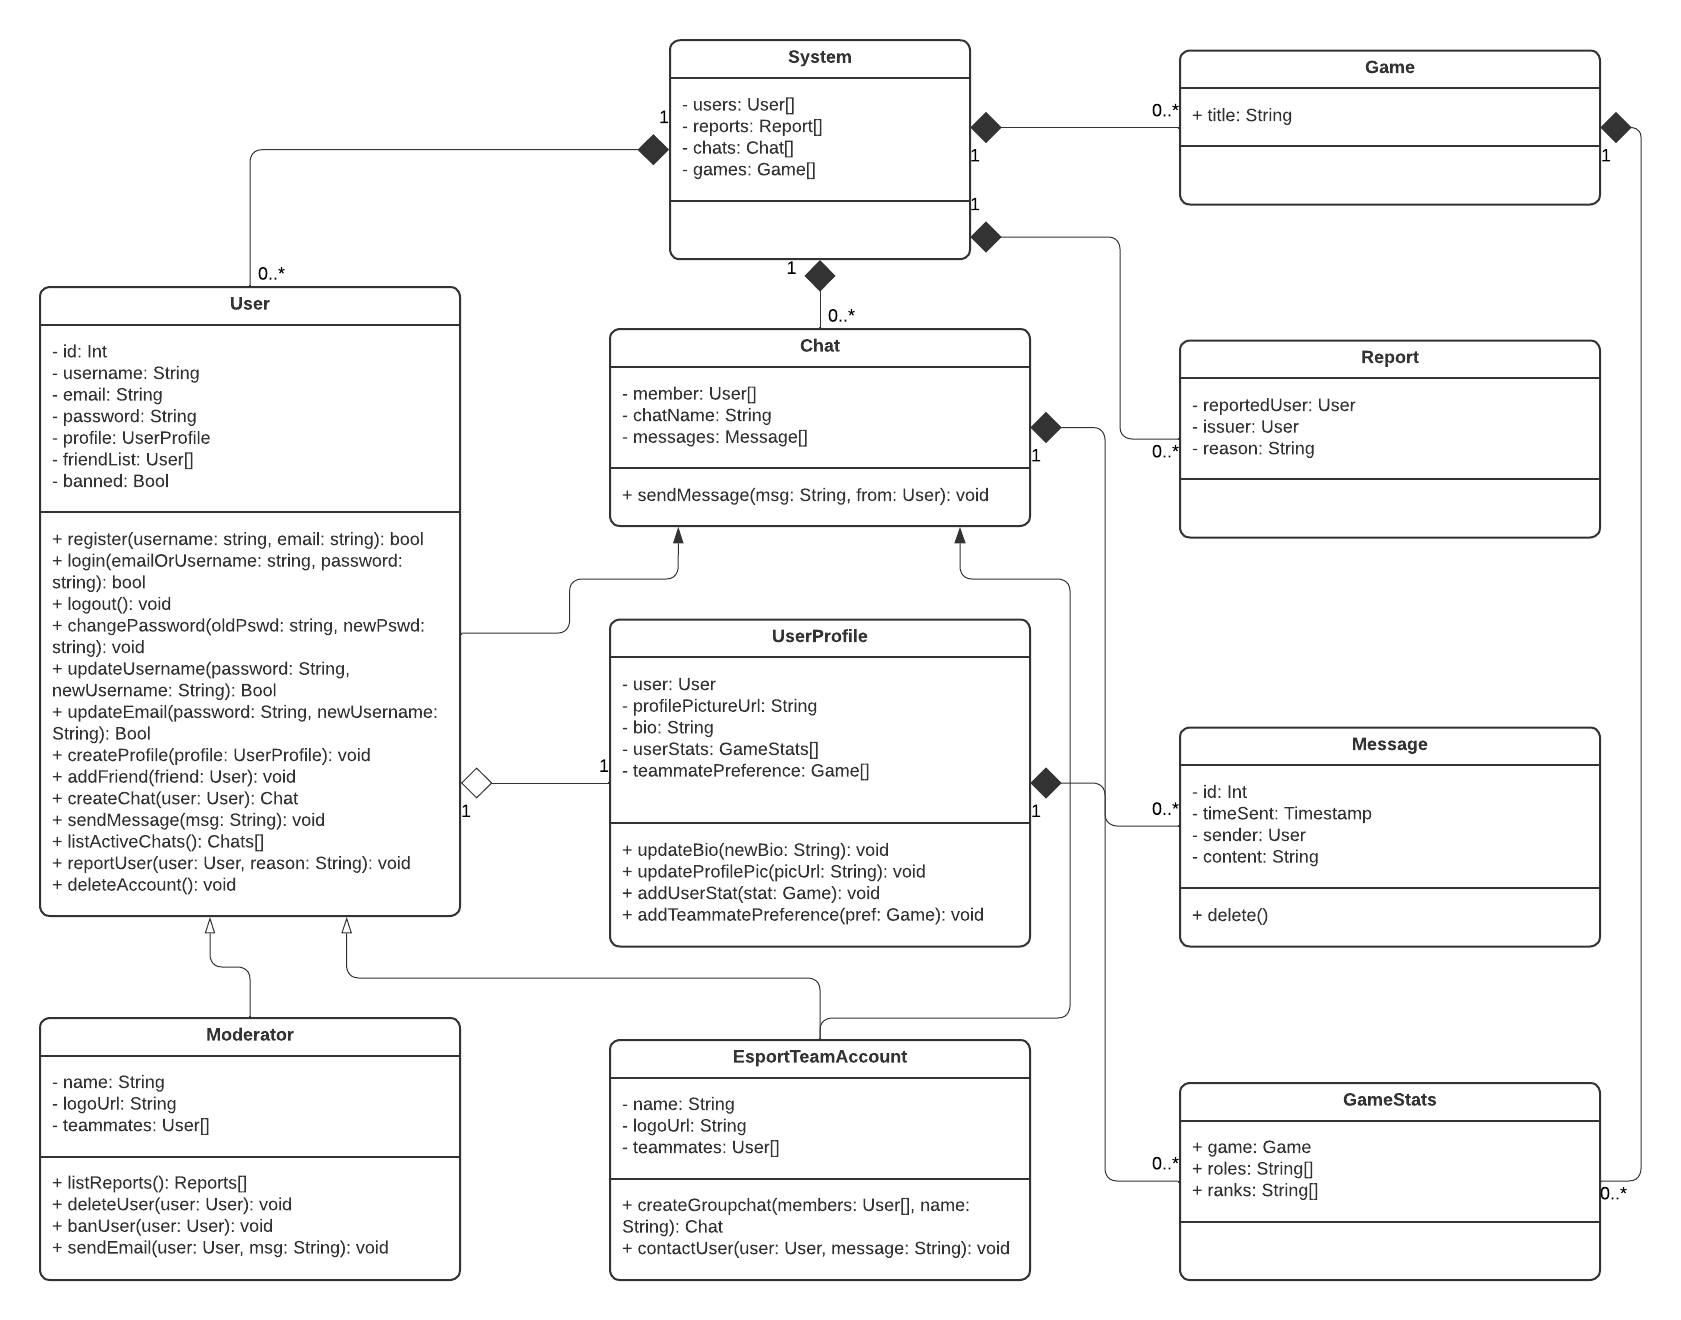
\includegraphics[width=1\textwidth, center]{Class_diagram.png}

\clearpage

\subsection{Sekvenční diagramy}
\subsubsection{Tvorba uživatelského profilu}

Sekvenční diagram popisující tvorbu uživatelského profilu.

\bigskip
\bigskip
\bigskip
\bigskip
\bigskip
\bigskip


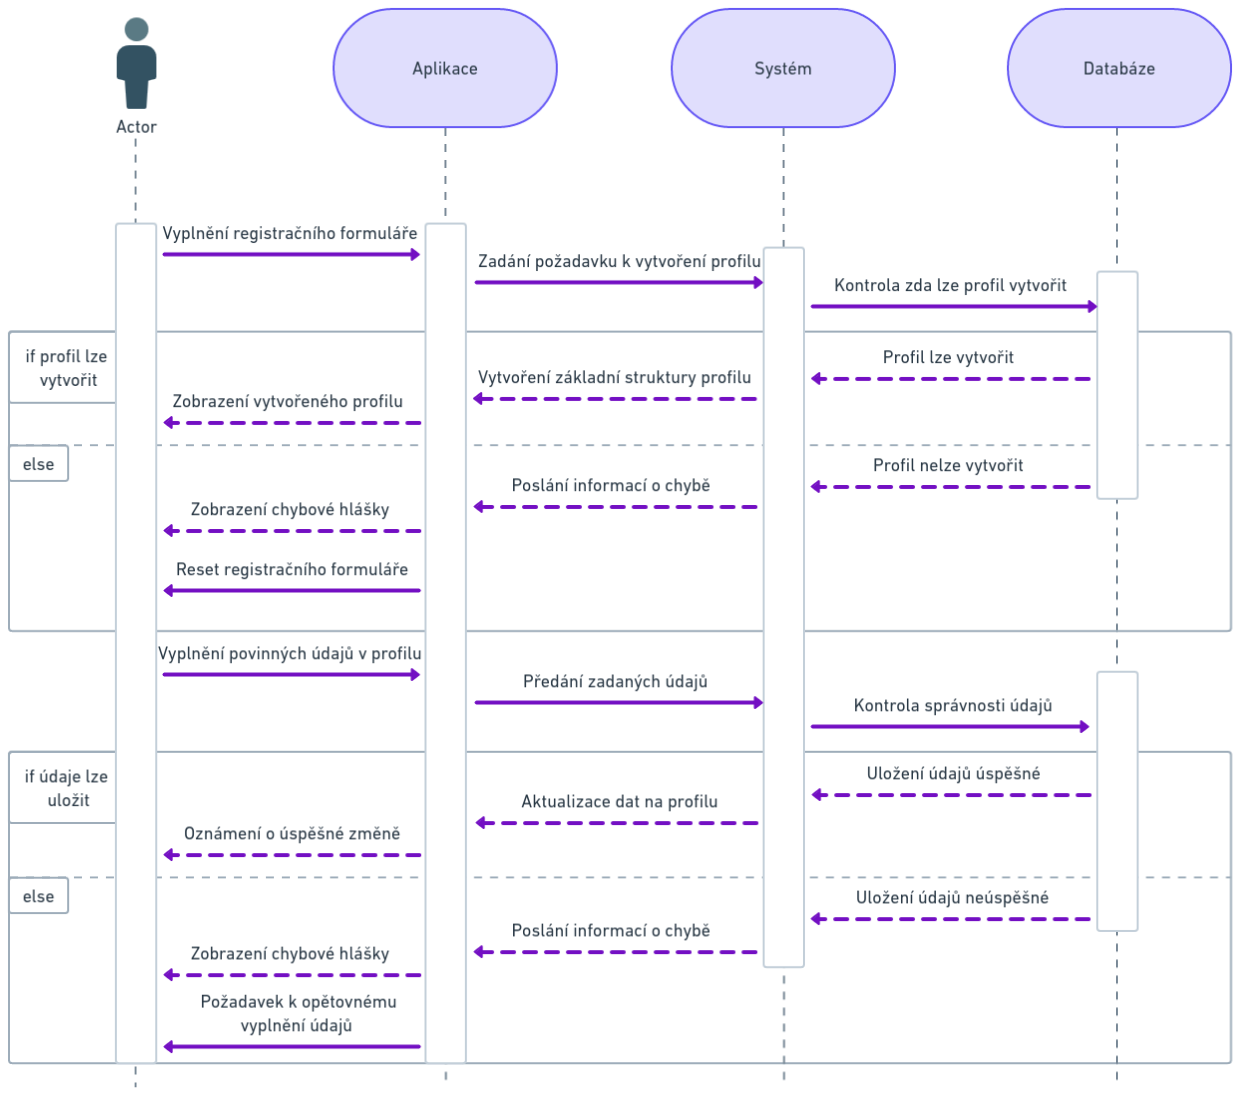
\includegraphics[width=1\textwidth, center]{Sequence_diagram _1.png}

\clearpage

\subsubsection{Hledání shody}

Sekvenční diagram popisující hledání shody s jiným uživatelem.

\bigskip
\bigskip
\bigskip
\bigskip
\bigskip
\bigskip


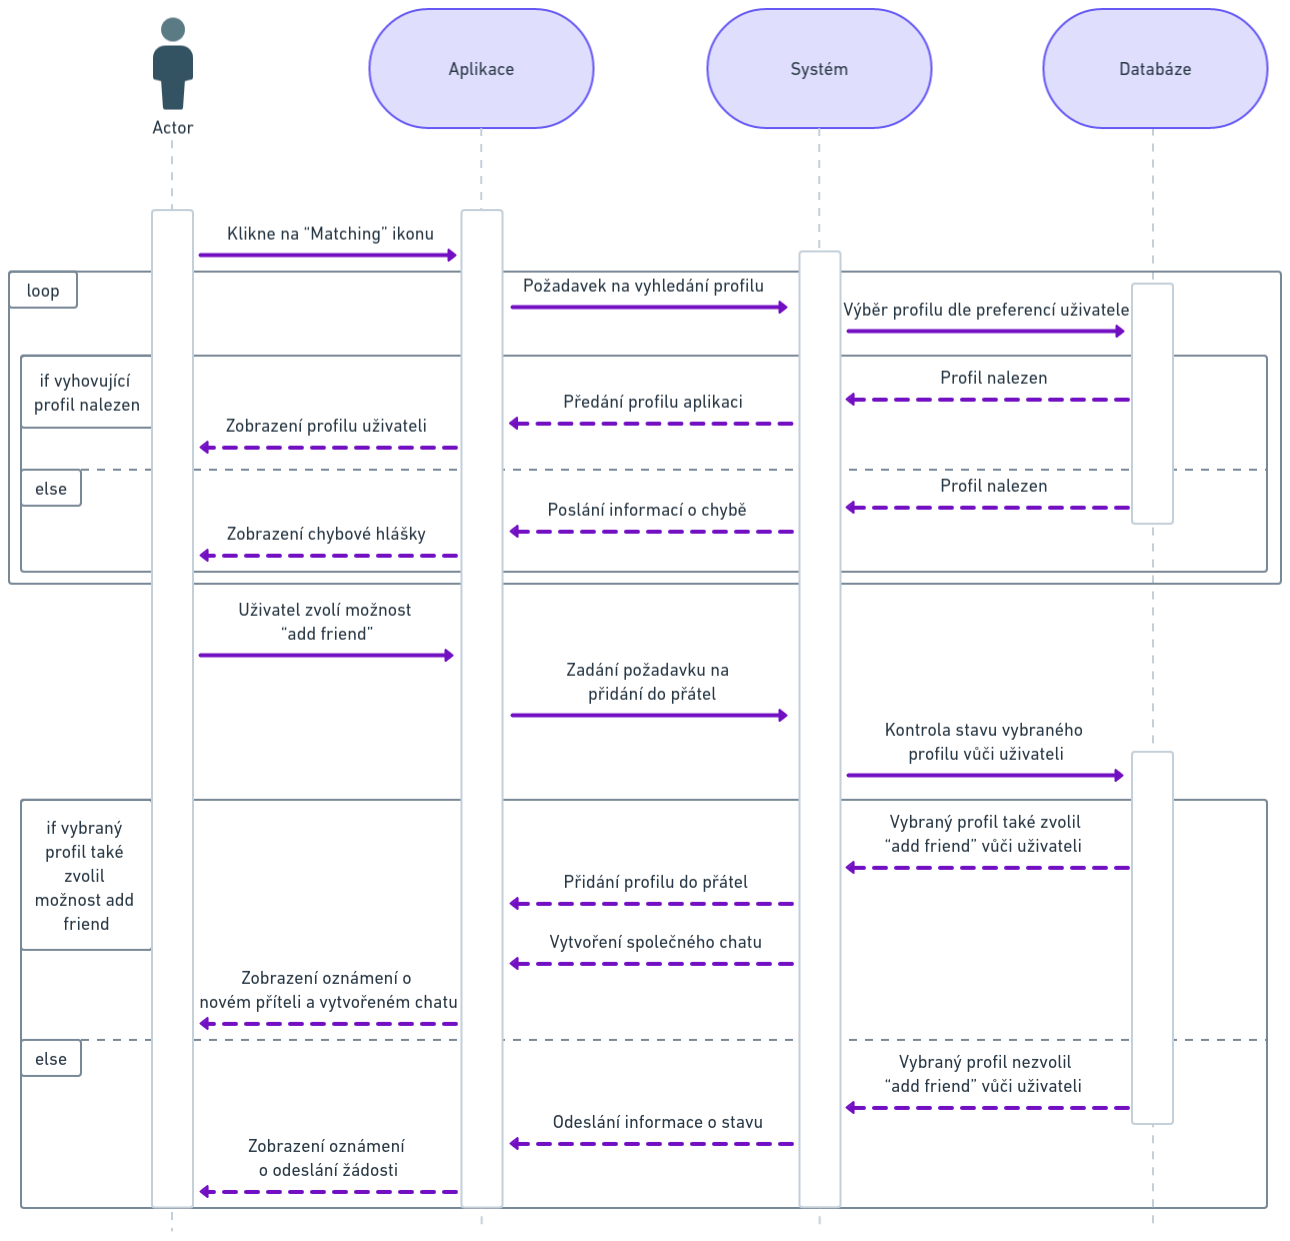
\includegraphics[width=1\textwidth, center]{Sequence_diagram _2.png}

\clearpage

\subsubsection{Založení group chatu}

Sekvenční diagram popisující založení skupinového chatu e-sport teamem.

\bigskip
\bigskip
\bigskip
\bigskip
\bigskip
\bigskip


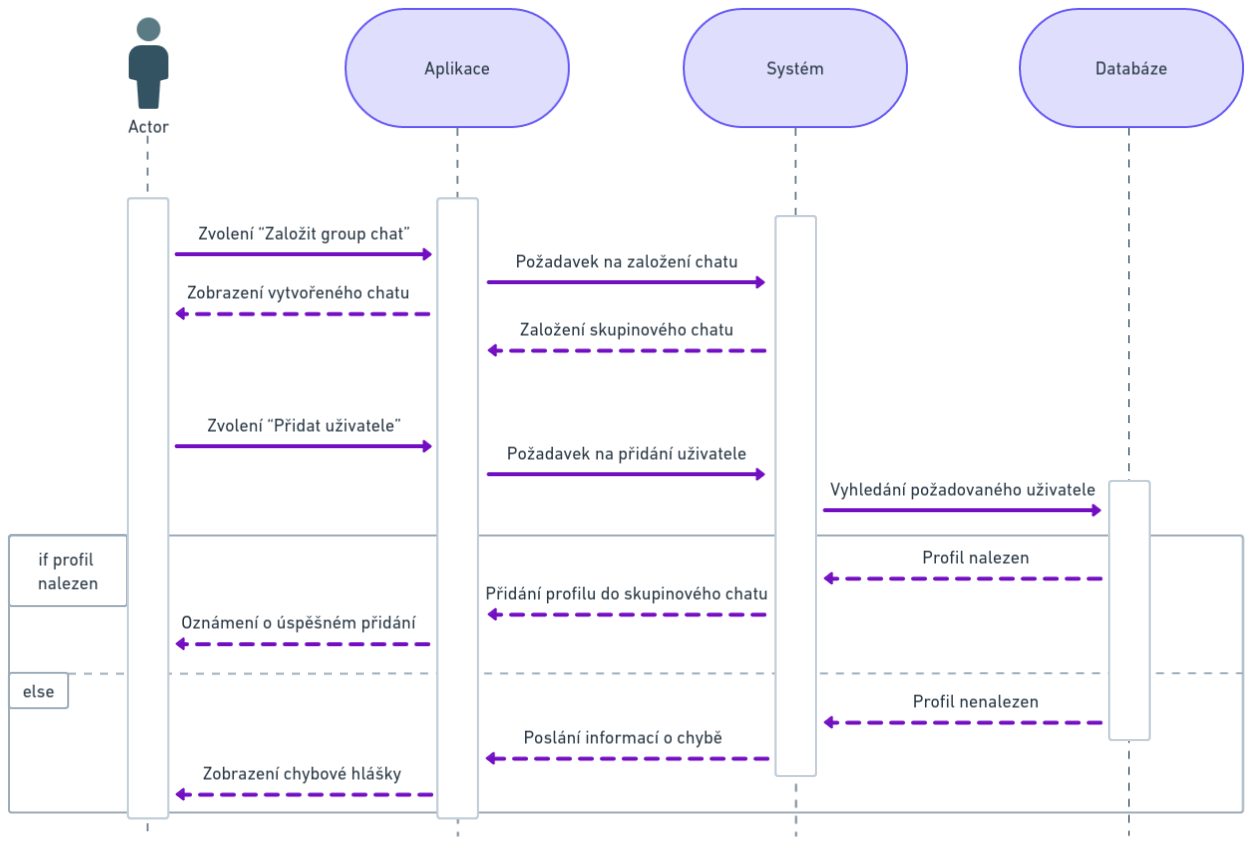
\includegraphics[width=1\textwidth, center]{Sequence_diagram _3.png}

\clearpage

\subsection{Aktivitní diagramy}
\subsubsection{Registrace uživatele}

Aktivitní diagram reprezentující proces registrace uživatele.

\bigskip
\bigskip
\bigskip
\bigskip
\bigskip
\bigskip


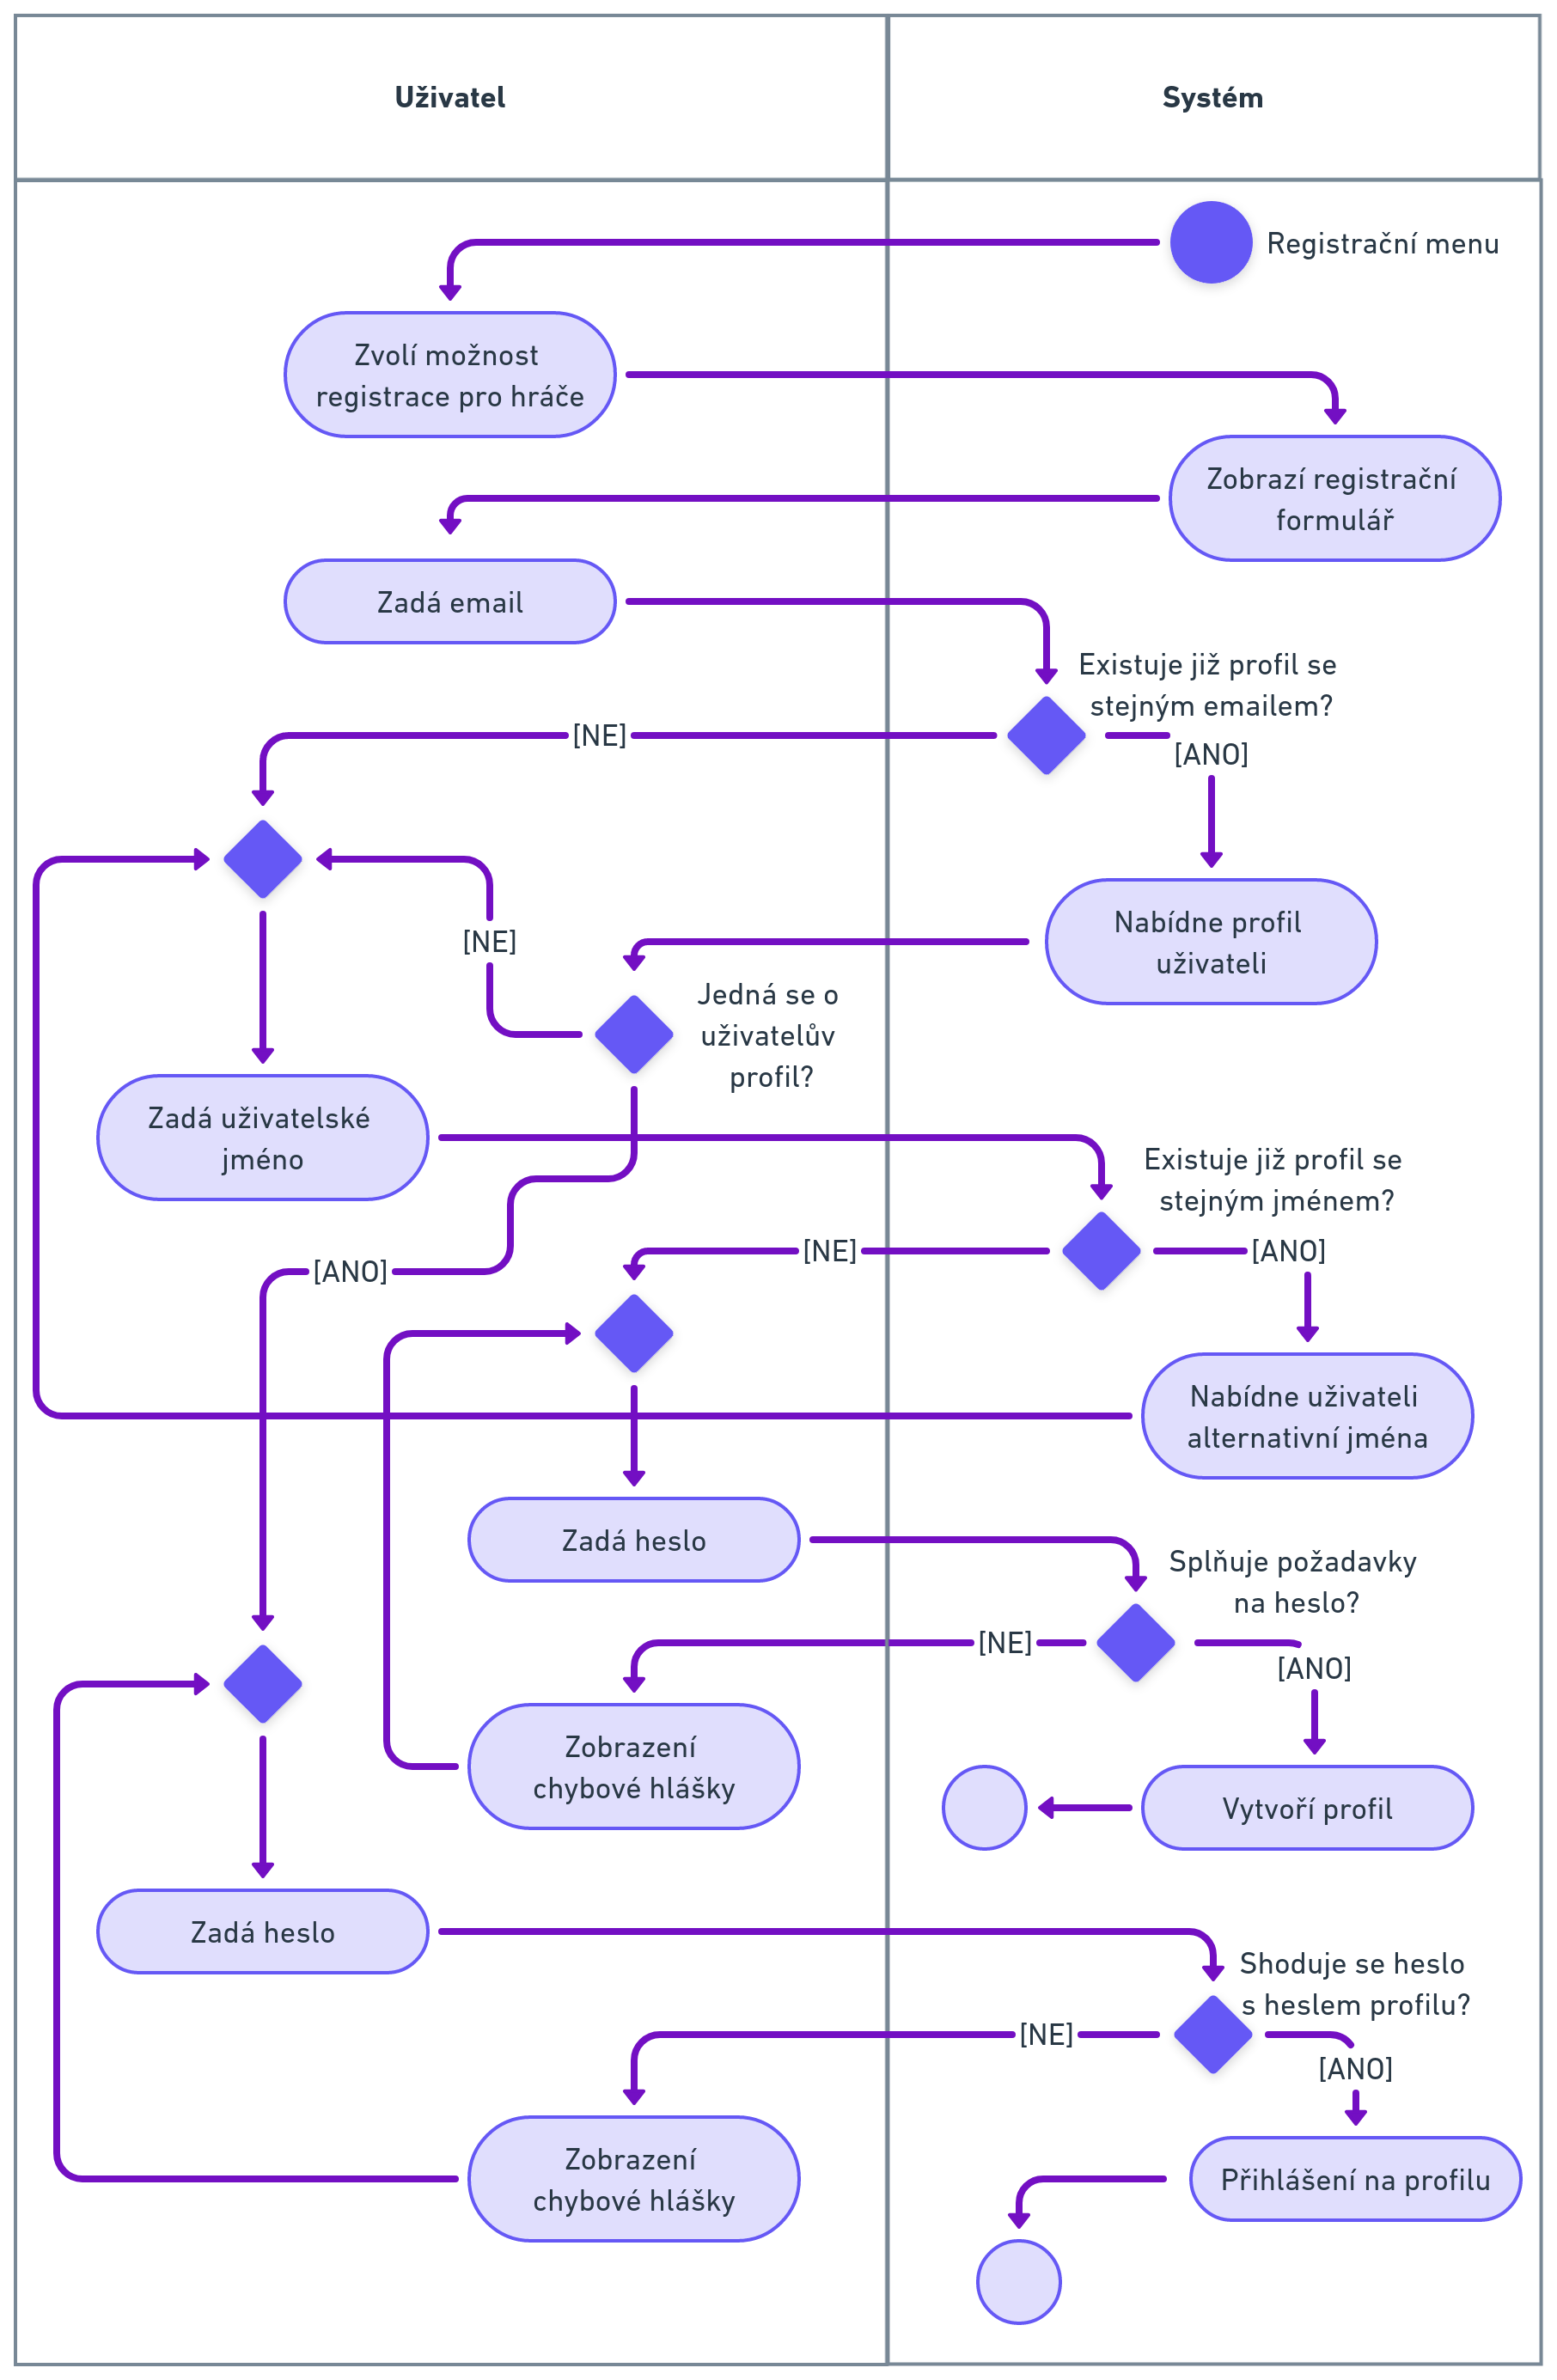
\includegraphics[width=0.8\textwidth, center]{Activity_diagram_1.png}

\clearpage

\subsubsection{Nahlášení profilu}

Aktivitní diagram reprezentující proces řešení nahlášení uživateleského profilu.

\bigskip
\bigskip
\bigskip
\bigskip
\bigskip
\bigskip

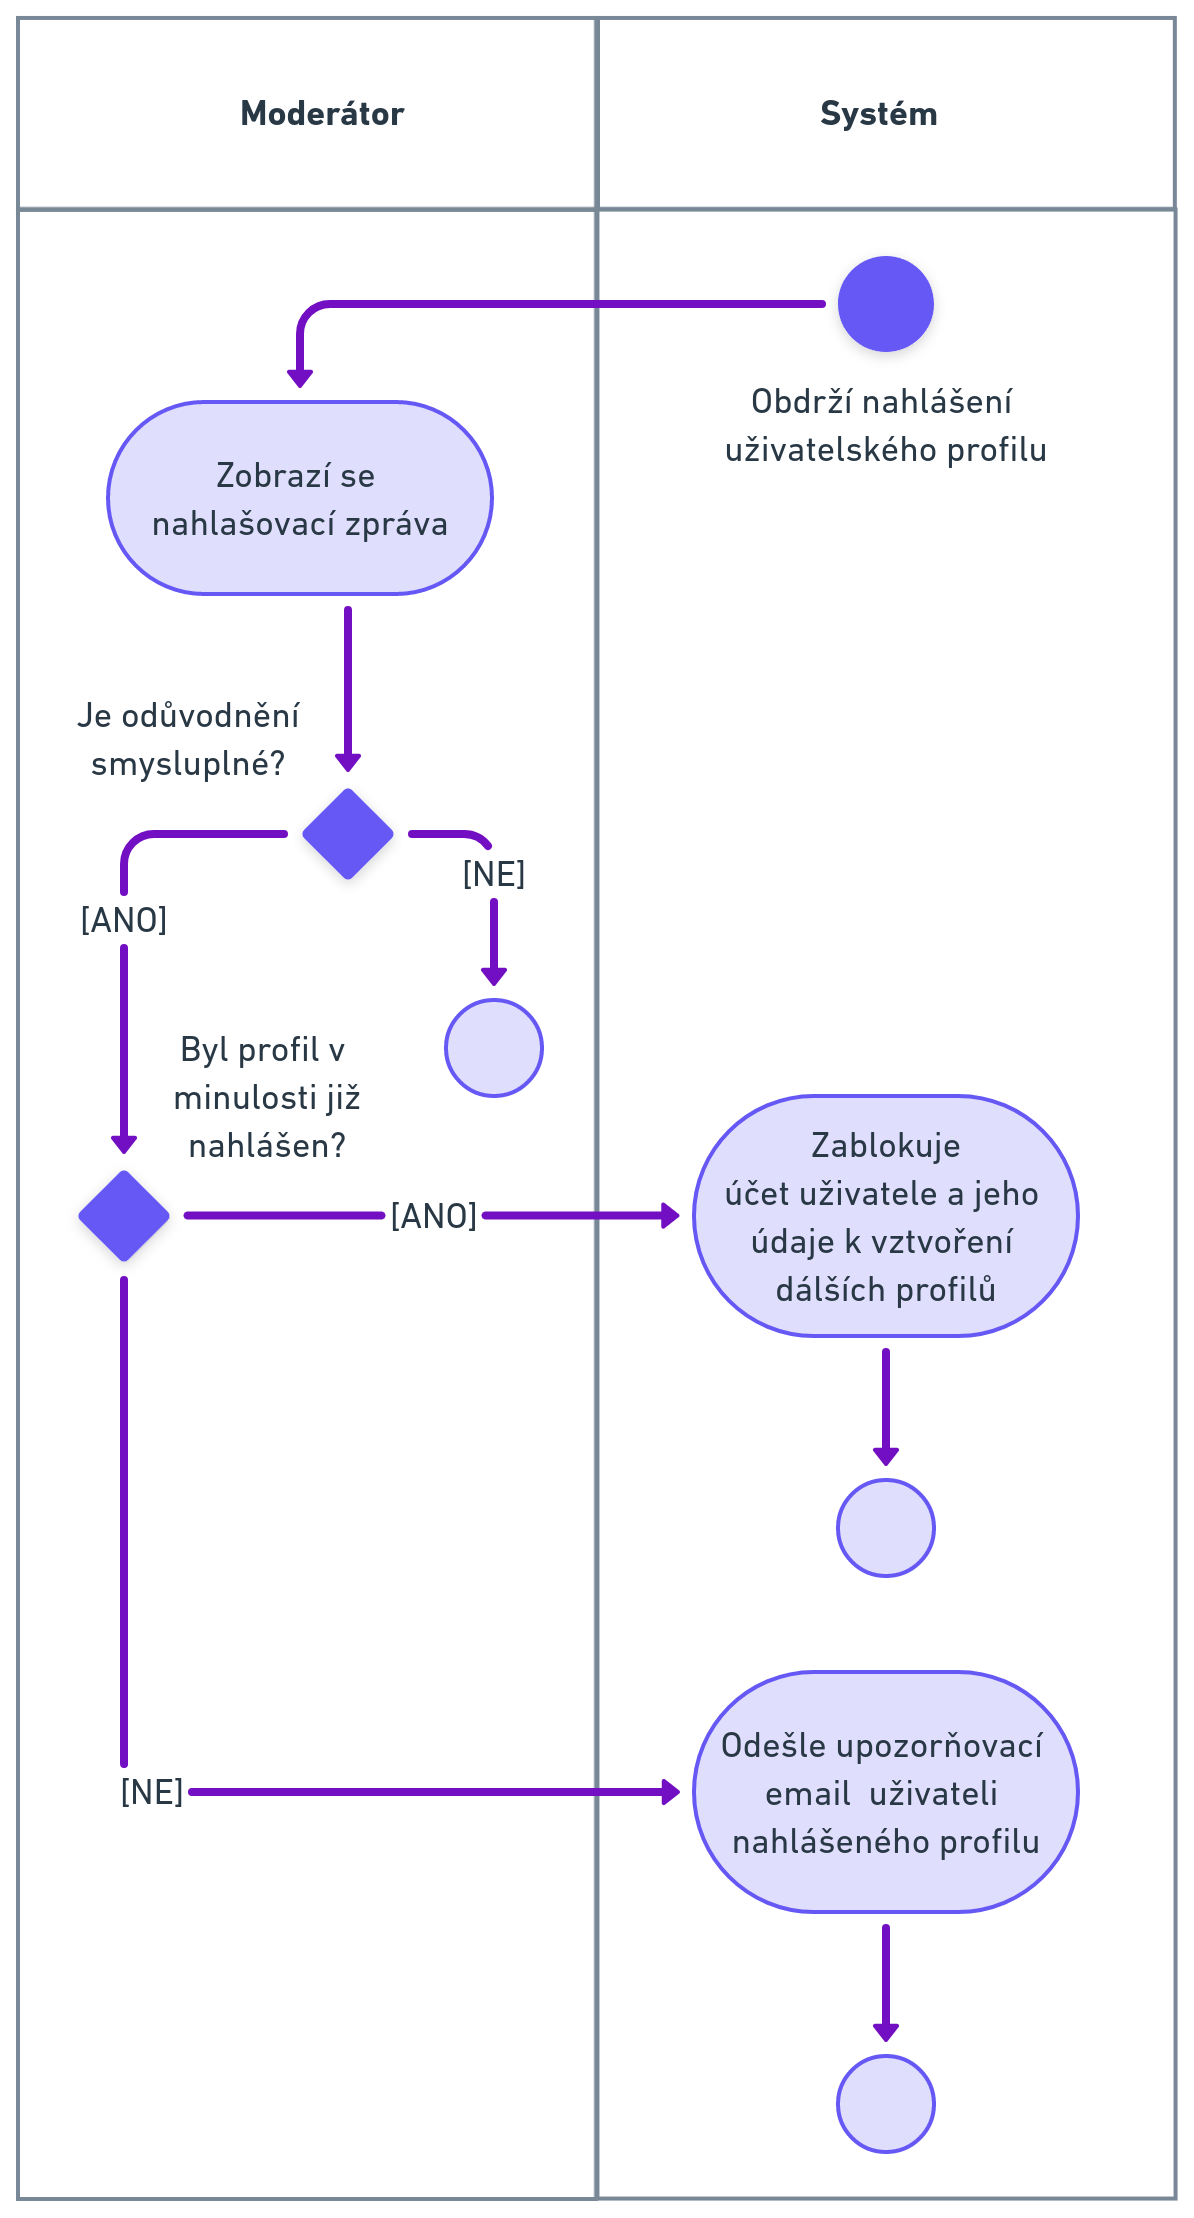
\includegraphics[width=0.6\textwidth, center]{Activity_diagram_2.png}

\clearpage

\subsubsection{Založení group chatu}

Aktivitní diagram reprezentující proces vytvoření skupinového chatu.

\bigskip
\bigskip
\bigskip
\bigskip
\bigskip
\bigskip


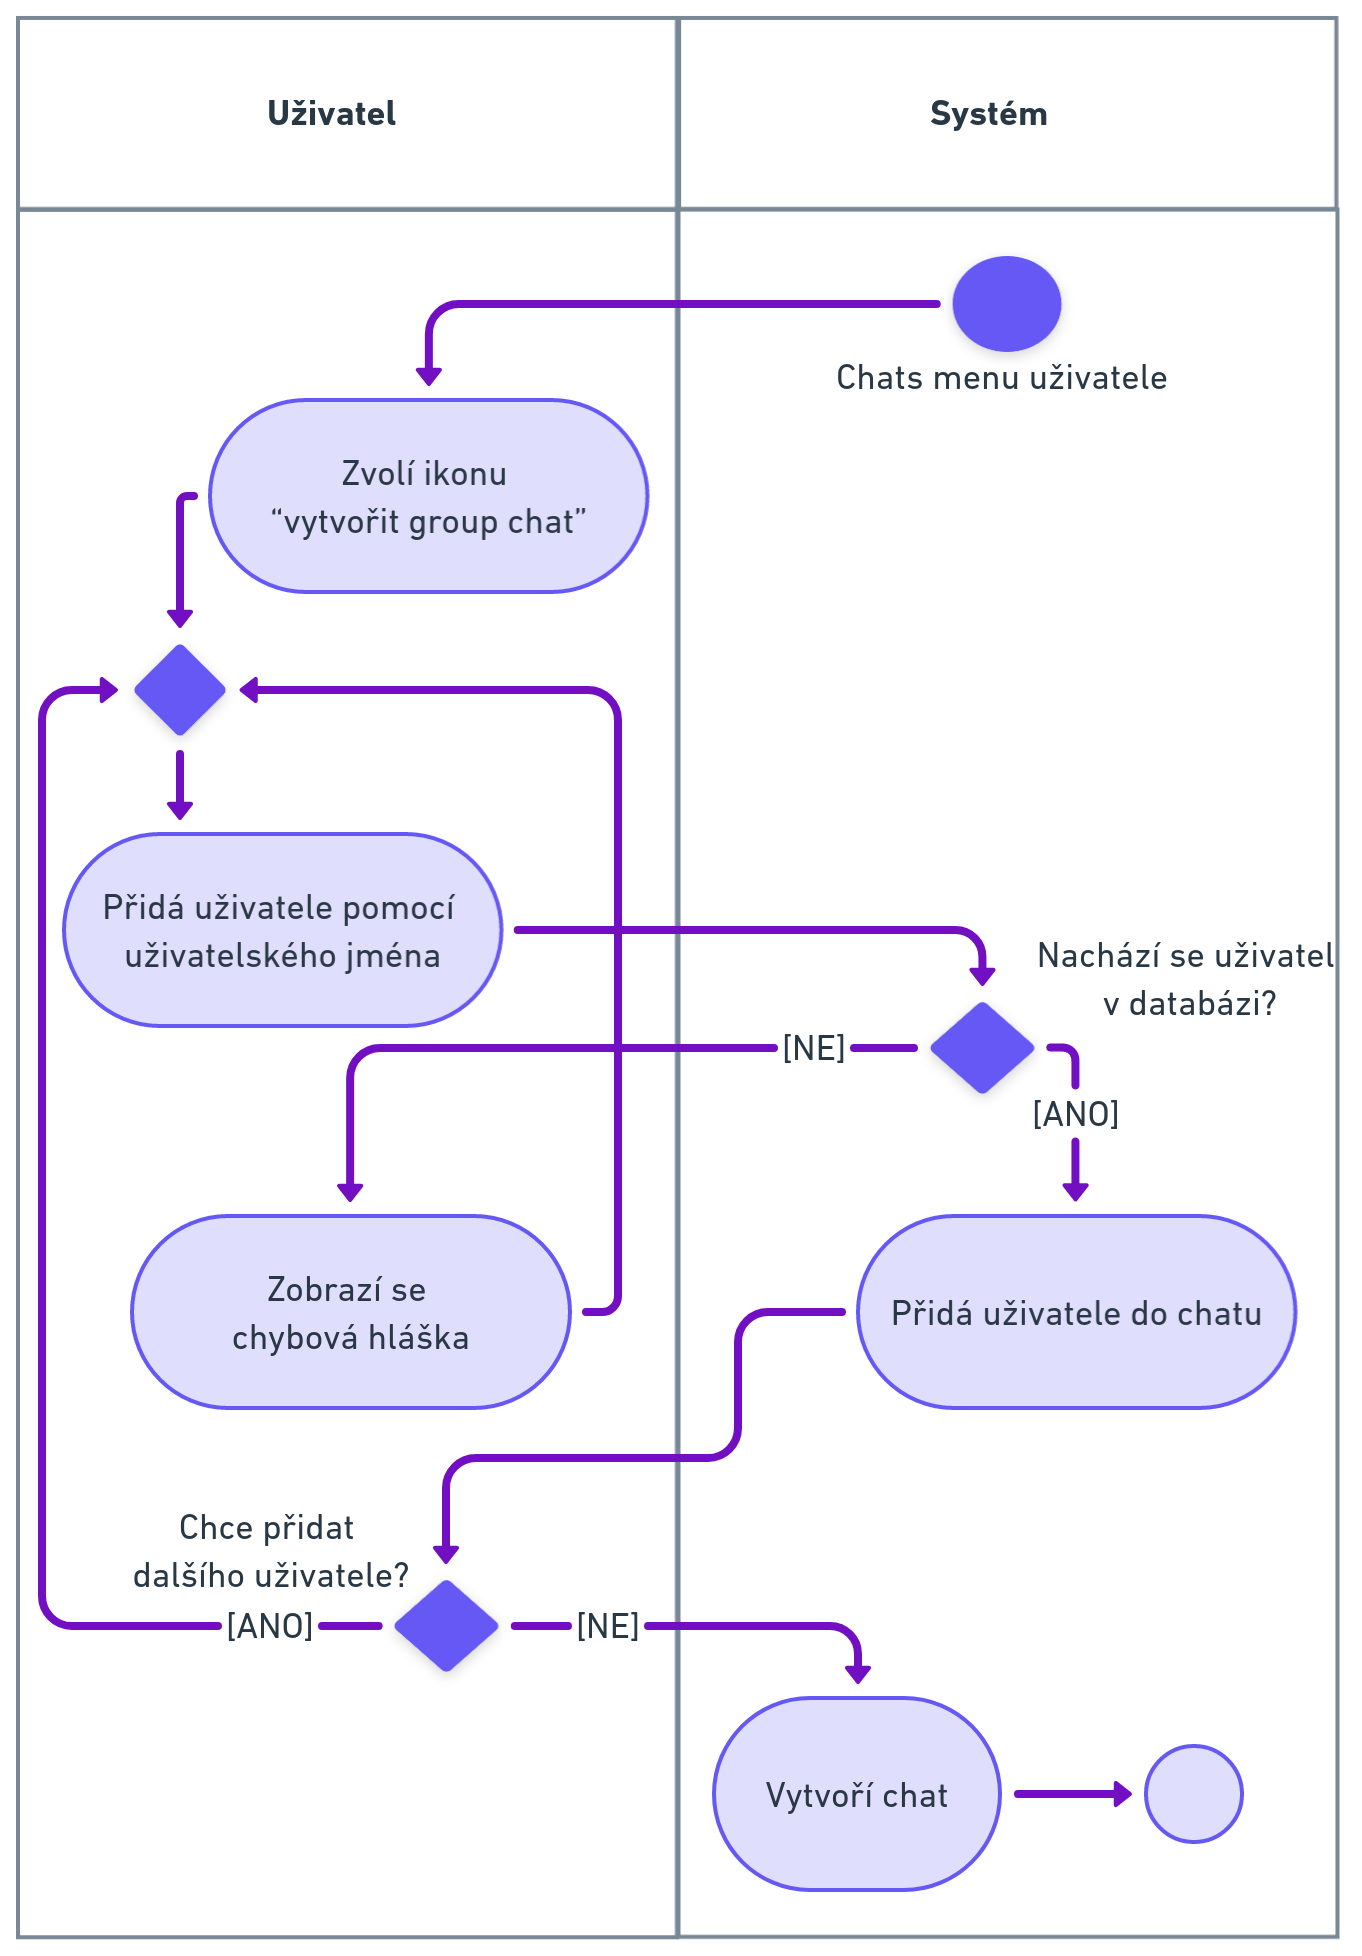
\includegraphics[width=0.8\textwidth, center]{Activity_diagram_3.png}

\clearpage

\subsection{Stavové diagramy}
\subsubsection{Odesílání zpráv}

\bigskip
\bigskip
\bigskip
\bigskip
\bigskip
\bigskip


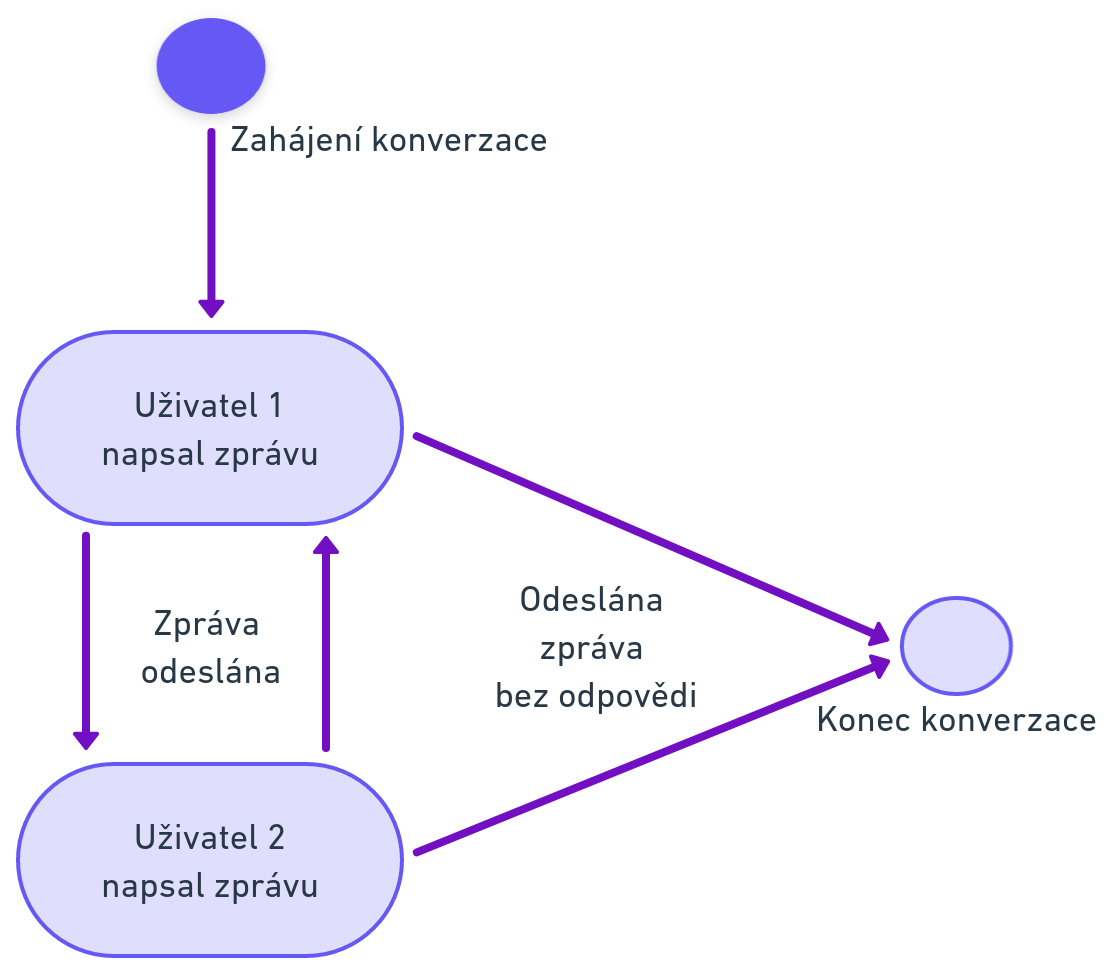
\includegraphics[width=0.65\textwidth, center]{State_diagram_1.png}

\clearpage

\subsubsection{Vytvoření skupinového chatu}

\bigskip
\bigskip
\bigskip
\bigskip
\bigskip
\bigskip


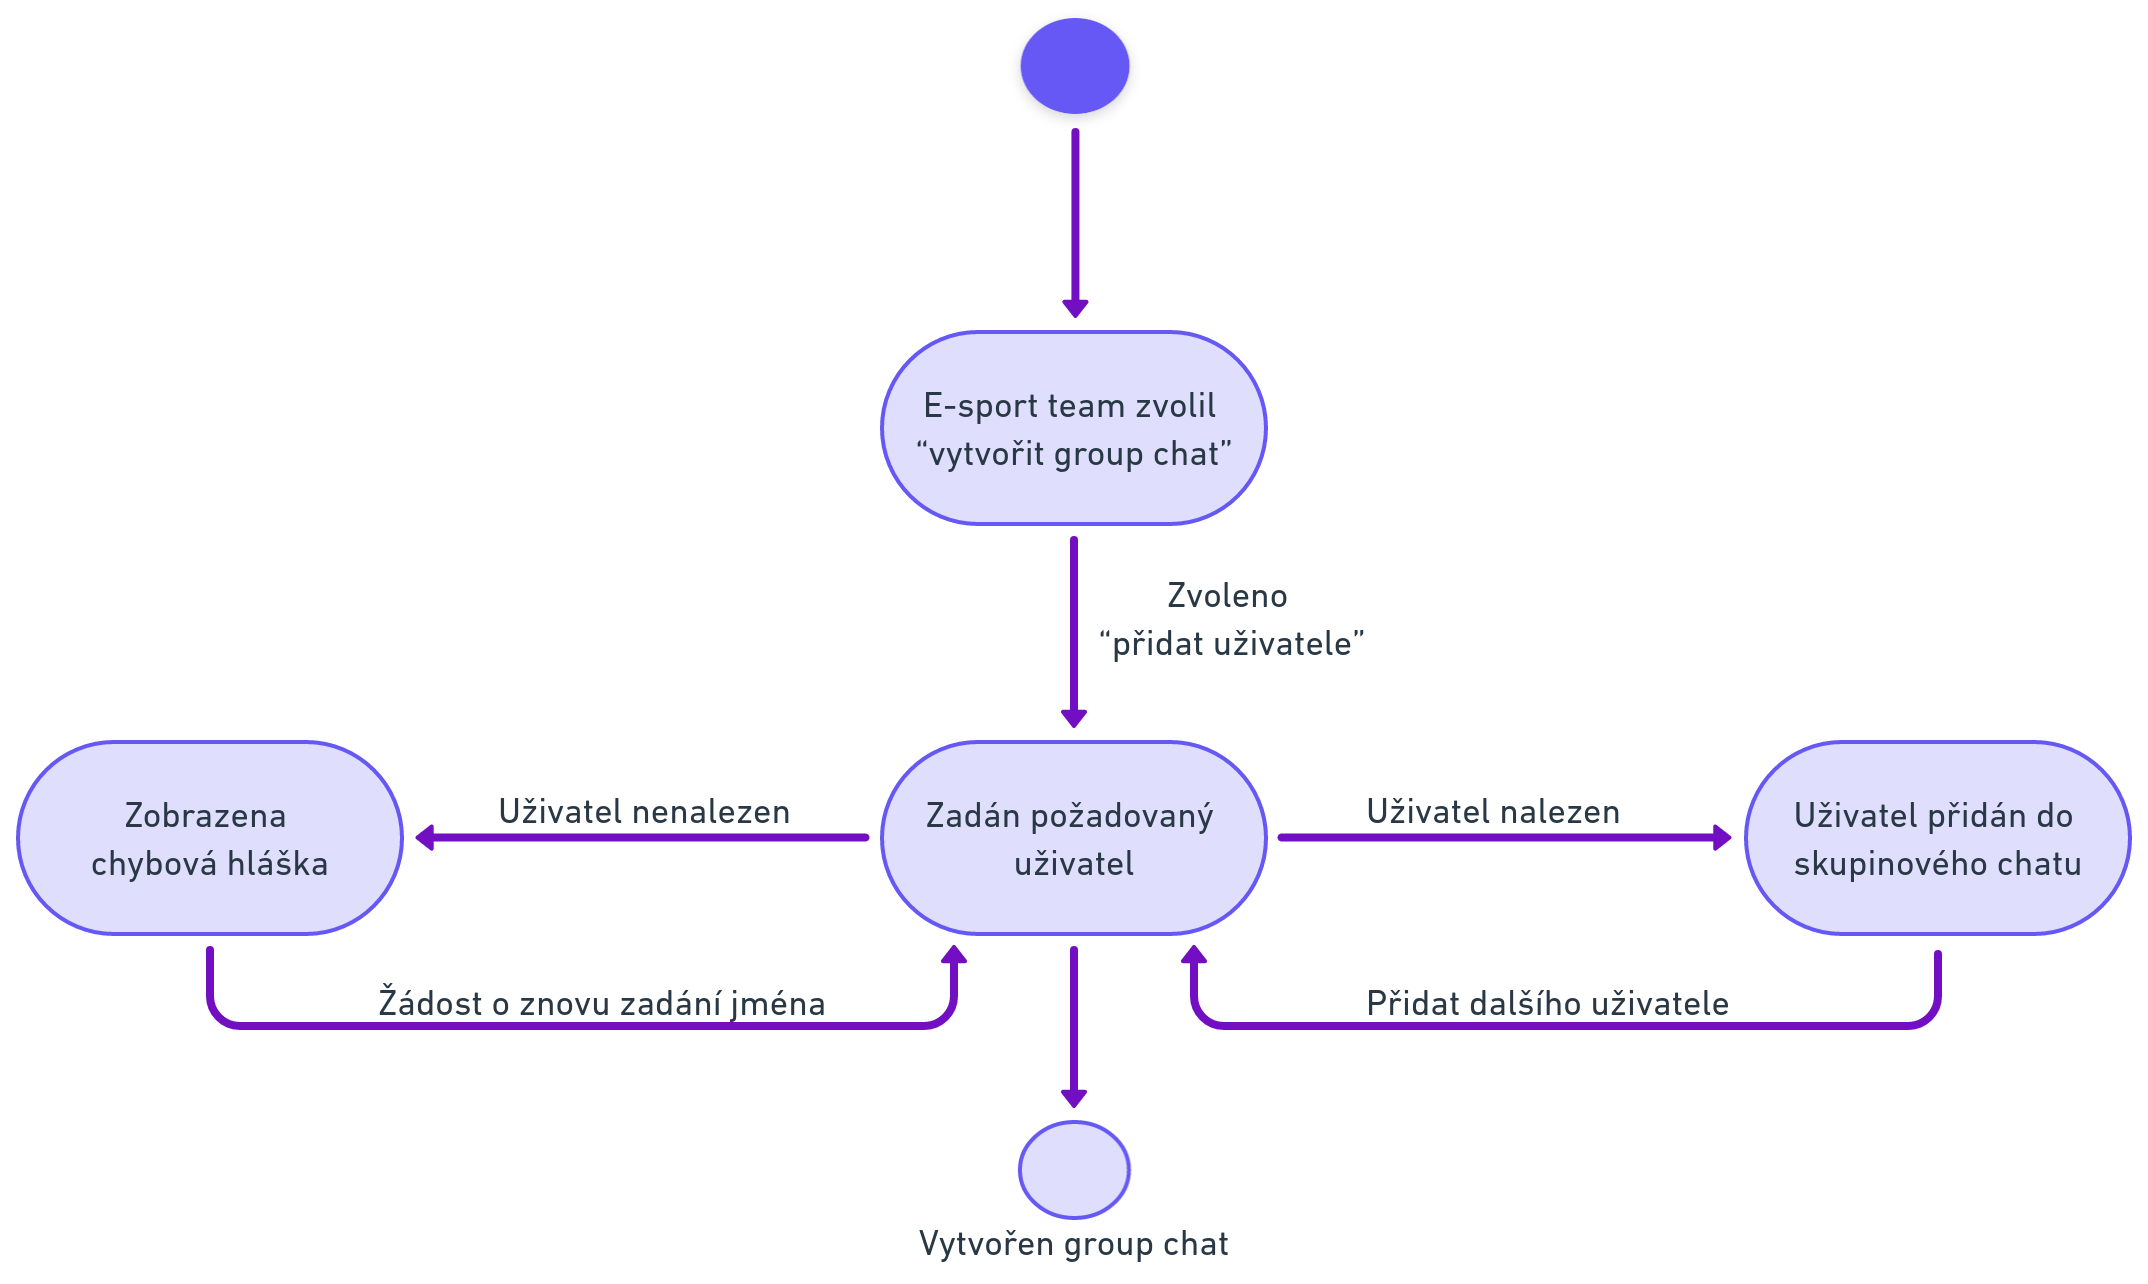
\includegraphics[width=1\textwidth, center]{State_diagram_2.png}

\clearpage

\subsubsection{Provoz}

Nemohla jsem najít situaci tohoto projektu, pro kterou bych mohla vytvořit
stavový diagram, proto jsem si vybrala nějakou mimo tento projekt.

\bigskip
\bigskip
\bigskip
\bigskip
\bigskip
\bigskip


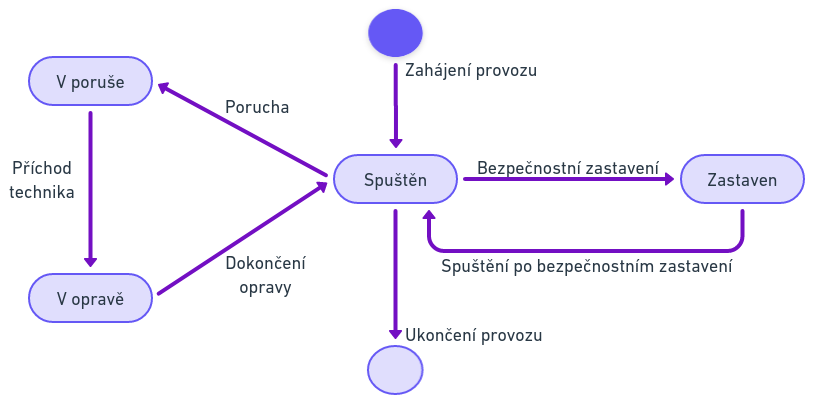
\includegraphics[width=1\textwidth, center]{State_diagram_3.png}

\clearpage

\end{document}